\hypertarget{ux5de5ux5177ux8c03ux7528}{%
\chapter{工具调用}\label{ux5de5ux5177ux8c03ux7528}}

\hypertarget{ux5de5ux5177ux8c03ux7528-1}{%
\section{工具调用}\label{ux5de5ux5177ux8c03ux7528-1}}

为了让大语言模型成为从单纯的``大脑''变为能实时感知并执行任务的智能体，我们需要让它具备调用工具的能力，具体包括以下方面。

\hypertarget{ux4e00ux5de5ux5177ux8c03ux7528ux7684ux57faux672cux6d41ux7a0bux4e0eux7b56ux7565}{%
\subsection{一、工具调用的基本流程与策略}\label{ux4e00ux5de5ux5177ux8c03ux7528ux7684ux57faux672cux6d41ux7a0bux4e0eux7b56ux7565}}

\begin{enumerate}
\def\labelenumi{\arabic{enumi}.}
\item
  基本流程：判断是否需要使用工具---选择合适的工具---调用工具---解析输出结果。
\item
  策略
\end{enumerate}

（1）提示词驱动：如加入prompt``如果你觉得当前知识不足或需要实时信息，请使用对应工具。如果你可以直接回答，就直接生成答案。''提示词中一般会加入可用的工具定义；考虑到上下文有限，实际上一般只加入``元工具''的定义（如bash命令，模型通过运行命令可以调用其他次级工具），或只放工具列表（模型在需要时自主至文件系统搜索工具）。

（2）ReAct范式（Reason + Act）

前面讲了用提示词驱动大模型使用工具，也讲过推理中的思维链，但这两者是并行的，它们之间并没有很好地协同。ReAct范式则将它们结合起来，比如下面的例子：

Question: 一美元等于多少日元？

Thought: 我不知道当前汇率，应该先查一下。

Action: SEARCH{[}一美元对日元汇率{]}

Observation: 当前汇率为 157.5

Thought: 得到了汇率，现在可以计算。

Action: CALC{[}157.5 × 20{]}

Observation: 结果为 3150

Final Answer: 20美元约等于3150日元。

当然，本质上这还是用提示词实现的。

（3）通过RL训练，让模型自主学会在合适的时候调用工具。

\hypertarget{ux4e8cux5de5ux5177ux7684ux7c7bux522b}{%
\subsection{二、工具的类别}\label{ux4e8cux5de5ux5177ux7684ux7c7bux522b}}

\begin{enumerate}
\def\labelenumi{\arabic{enumi}.}
\item
  信息检索类工具：对应人的``感知神经元''，帮助模型实时获得信息或知识，如搜索引擎、知识数据库、上传文档的解析工具等。
\item
  计算推理类工具：对应人的``中枢神经元''，帮助模型精确运算或推理，避免基于概率的大模型自身推理中可能出现的错误，如计算器、代码解释器等。
\item
  设备控制类工具：对应人的``运动神经元''，帮助模型在实际环境中执行任务，如控制操作系统、应用程序、机器人等的工具。
\end{enumerate}

\hypertarget{ux4e09ux5de5ux5177ux7684ux63a5ux53e3}{%
\subsection{三、工具的接口}\label{ux4e09ux5de5ux5177ux7684ux63a5ux53e3}}

为了让模型理解工具的用途、调用方式等，我们需要设计特定的API接口，以用模型能理解的形式将它们封装起来。工具接口需要有工具名称、用途描述、输入参数，以及对输入参数中有哪些必须填写的说明。

\hypertarget{ux56dbux591aux79cdux5de5ux5177ux7684ux6574ux5408}{%
\subsection{四、多种工具的整合}\label{ux56dbux591aux79cdux5de5ux5177ux7684ux6574ux5408}}

\begin{enumerate}
\def\labelenumi{\arabic{enumi}.}
\item
  工具的选择：可以在提示中提供工具列表，或设置一个关键词触发路由等。
\item
  工具优先级与回退机制：优先调用一些成功率更高或代价更低的工具；如果调用失败，切换至优先级更低的工具；失败若干次，则直接回答，避免陷入死循环。还可以引入反思机制，鼓励模型评估失败原因并改进下一步调用。
\end{enumerate}

\hypertarget{ux4e94ux5de5ux5177ux8fd4ux56deux7ed3ux679cux7684ux538bux7f29}{%
\subsection{五、工具返回结果的压缩}\label{ux4e94ux5de5ux5177ux8fd4ux56deux7ed3ux679cux7684ux538bux7f29}}

工具返回的结果有时候巨大无比，会占满上下文空间。此时可以采取剪枝方式，压缩时间靠前的输出后再输入给LLM。这个压缩是有损过程，但这个过程不重写硬盘中的返回结果文件。

\hypertarget{ux516dux601dux7ef4ux4e0aux4e0bux6587ux7ba1ux7406ux89e3ux51b3ux8c03ux7528ux5de5ux5177ux540eux7684ux63a8ux7406ux65adux94fedeepseek2025}{%
\subsection{六、思维上下文管理：解决调用工具后的推理``断链''（DeepSeek，2025）}\label{ux516dux601dux7ef4ux4e0aux4e0bux6587ux7ba1ux7406ux89e3ux51b3ux8c03ux7528ux5de5ux5177ux540eux7684ux63a8ux7406ux65adux94fedeepseek2025}}

常见的含工具调用的推理模型的工作流往往是：用户问题~-\textgreater{} 模型``内部思考''（状态A）-\textgreater{} 执行工具 -\textgreater~工具结果 + 用户问题~-\textgreater{} 模型``内部思考''（状态B）。在进入状态B时，状态A并没有被保存起来。

DeepSeek设计了一套让模型能像人类一样``参考笔记''来完成复杂任务的机制。V3.2的流程是：用户问题~-\textgreater{} 模型生成~reasoning\_content\_A（写在``草稿纸''上）-\textgreater{} 执行工具 -\textgreater~工具结果 + 用户问题 +~reasoning\_content\_A（作为上下文输入）~-\textgreater{} 模型基于之前的``草稿''继续推理，生成~reasoning\_content\_B。

\hypertarget{ux53c2ux8003ux6587ux732e-120}{%
\subsection{参考文献}\label{ux53c2ux8003ux6587ux732e-120}}

\begin{itemize}
\tightlist
\item
  《动手学大模型智能体》。
\item
  Yao, S., Zhao, J., Yu, D., et al.~(2023). \href{https://arxiv.org/abs/2210.03629}{ReAct: Synergizing Reasoning and Acting in Language Models}. ICLR 2023.
\item
  DeepSeek-AI. (2025). \href{https://arxiv.org/abs/2512.02556}{DeepSeek-V3.2: Pushing the Frontier of Open Large Language Models}. arXiv:2512.02556.
\end{itemize}

\clearpage

\hypertarget{ux6a21ux578bux4e0aux4e0bux6587ux534fux8bae}{%
\section{模型上下文协议}\label{ux6a21ux578bux4e0aux4e0bux6587ux534fux8bae}}

模型上下文协议（Model Context Protocol，简称MCP）是由Anthropic于2024年11月推出的一项开源标准协议。它是模型侧和工具侧之间的协议，核心目标是为大型语言模型（LLM）提供一个标准化的接口，使其与外部数据源、工具和开发环境的接口匹配，主要在AI调用外部工具或读取外部工具时使用（如果工具代码或数据库读取代码已经全部封装在模型侧，就不需要）。

如果打个比方，MCP就像是AI界的``USB-C接口''。正如USB-C统一了各种电子设备的物理连接方式一样，MCP统一了AI应用与外部世界（如本地文件系统、企业数据库、API 服务等）的连接和交互标准。

\hypertarget{ux4e00ux4ea7ux751fux80ccux666f-1}{%
\subsection{一、产生背景}\label{ux4e00ux4ea7ux751fux80ccux666f-1}}

大模型走向Agent，一个重要的问题是许多外部工具或私有数据是由对应领域的企业封装的，需要让模型厂商的模型侧接口和外部企业提供的接口匹配，才能调用这些工具，而不同的模型厂商（如 OpenAI、Anthropic、Google）有各自实现工具调用的数据结构。开发者如果想让一个内部的数据库查询工具同时支持GPT和Claude，必须编写和维护多套适配层代码。

MCP 通过定义一套独立于模型厂商的通用协议，实现了``一次开发，多模运行''。工具开发者只需按照MCP标准封装一次系统能力，即可被任何支持该协议的AI客户端统一调度。

\hypertarget{ux4e8cux6838ux5fc3ux67b6ux6784-1}{%
\subsection{二、核心架构}\label{ux4e8cux6838ux5fc3ux67b6ux6784-1}}

\begin{figure}[htbp]
\centering
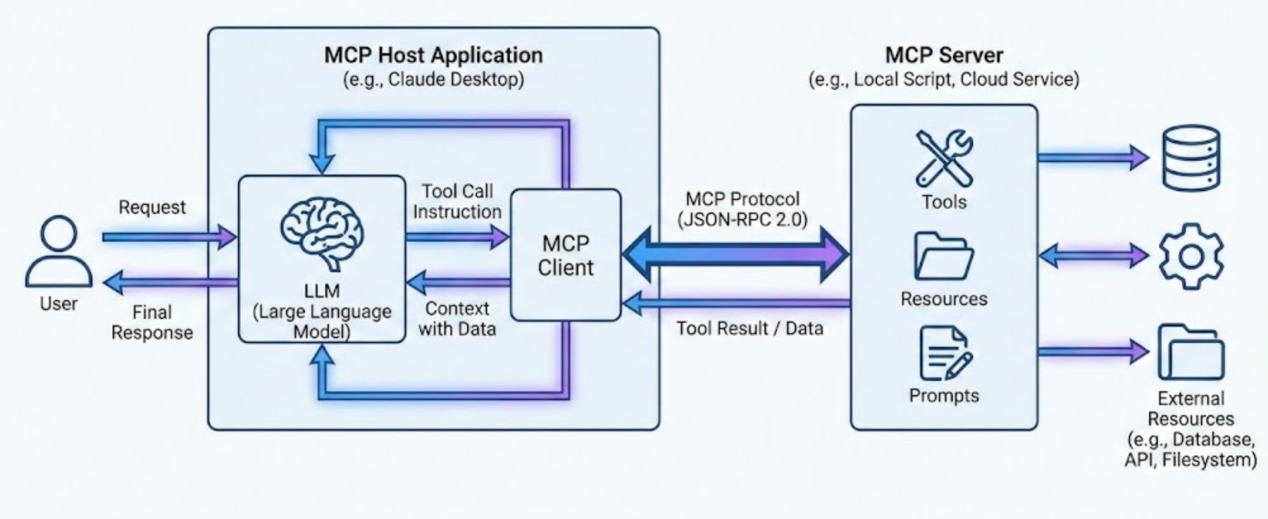
\includegraphics{images/image-0033.png}
\caption{MCP Host、Client、Server 与外部资源的交互架构}
\end{figure}

MCP Host：用户直接交互的AI应用程序或环境，例如Claude Desktop、Cursor等，在模型侧，内部运行着LLM。LLM需要调用工具时，Host根据LLM输出的调用工具名称，找到对应的MCP Client。

MCP Client（客户端）：嵌入在模型侧的Host内部，是LLM与外部资源之间的``翻译官''。每个Host中有多个Client，每个Client对应一种或多种工具、与负责该工具的Server保持一对一的连接。它负责将LLM的输出转换为符合MCP标准的结构化请求，管理网络会话状态，并处理工具调用的路由和错误反馈。

MCP Server（服务器）：轻量级的独立程序，在外部工具或数据侧。每一个服务器都对应着一项或多项具体的能力，包括工具（可以执行的动作或函数）和资源（只读）。它可以是本地脚本，也可以是云端服务。Server向Client暴露自身的工具和数据读取能力，并在接收到标准指令后执行相应操作，将格式化后的结果返回给Client。

\hypertarget{ux4e09ux5de5ux4f5cux6d41ux7a0b}{%
\subsection{三、工作流程}\label{ux4e09ux5de5ux4f5cux6d41ux7a0b}}

\begin{enumerate}
\def\labelenumi{\arabic{enumi}.}
\item
  能力协商与初始化：Host启动时，模型侧的Client与外部的Server建立连接。双方首先通过发送JSON-RPC消息进行握手，确认彼此支持的协议版本和能力基元。
\item
  能力发现：Client向Server发送请求，拉取该Server当前可用的Tools和Resources的详细描述列表（包括工具的名称、用途、参数Schema），并将其注入到LLM的上下文中。为了保证工具的可扩展性，避免上下文爆炸和尽量保证缓存命中，我们往往倾向于在这里使用``元工具''，如启动其他工具的bash命令，由它后续再导向其他具体场景的工具。
\item
  用户发起请求：用户向Host提出问题，例如：``帮我查一下昨天数据库里新增了多少付费用户，并生成一份总结''。
\item
  LLM决策与指令生成：Host将用户的问题连同Server提供的工具列表一并发送给大模型进行推理。LLM分析后判断需要使用``数据库查询''工具，于是生成符合Schema要求的工具调用指令。
\item
  路由与执行：Host根据指令，将其路由到内部对应的Client。Client接收到工具调用指令，将其封装为MCP标准请求发送给外部对应的Server。Server执行SQL查询并获取数据，然后将结果返回给模型侧的Client。
\item
  上下文回传与最终响应：Client将查询结果作为新的上下文信息补充给大模型。LLM基于这些真实取回的数据进行逻辑推理，生成自然语言回答，最终由Host展示给用户。
\end{enumerate}

\hypertarget{ux53c2ux8003ux6587ux732e-121}{%
\subsection{参考文献}\label{ux53c2ux8003ux6587ux732e-121}}

\begin{itemize}
\tightlist
\item
  Anthropic. (2024). \href{https://www.anthropic.com/news/model-context-protocol}{Introducing the Model Context Protocol}.
\end{itemize}

\clearpage

\hypertarget{skills}{%
\section{Skills}\label{skills}}

\hypertarget{ux4e00ux57faux672cux601dux60f3-2}{%
\subsection{一、基本思想}\label{ux4e00ux57faux672cux601dux60f3-2}}

Agent的skills，可以理解为它的``专项能力包''，是一组可复用的本地指令、工作流程、参考资料，必要时还会配套脚本、模板或工具约束。一个Agent在面对任务时，如果调用了合适的 skill，就不必每次都从零开始推理，而是能按照既定的稳定流程完成工作。

核心价值：

\begin{enumerate}
\def\labelenumi{\arabic{enumi}.}
\item
  能把经验固化下来，如固定步骤、常见陷阱和验证方法，保证反复一致地执行；
\item
  降低出错率，skill往往会明确告诉Agent该读哪些文件、按什么顺序操作、什么时候该停下来确认，所以比临时发挥更可靠；
\item
  提升效率，面对复杂任务时，Agent不需要重新组织全部流程，而是直接套用合适的 skill，把时间花在真正需要判断和创造的部分。
\end{enumerate}

一个好的skill，不只是``会做什么''，还应说明``为什么这样做、做到什么程度、如何验证结果''。这样一来，Agent的能力就不再是模糊的，而是可解释、可检查、可持续改进的。

\hypertarget{ux4e8cux7528skillsux5c01ux88c5ux5de5ux5177ux8c03ux7528ux63a5ux53e3}{%
\subsection{二、用skills封装工具调用接口}\label{ux4e8cux7528skillsux5c01ux88c5ux5de5ux5177ux8c03ux7528ux63a5ux53e3}}

如果用模型的Context Window直接存储工具信息，并把工具调用结果也放进上下文，那上下文会被塞满，效率低下。而且模型通过MCP调用工具时，仍然有时会出现输出格式对不上等情形。

我们可以用skills封装工具接口，具体而言，即让模型通过运行封装在skills里的代码（在必要的时候模型也会补充一些脚本），来实现工具调用，工具调用的结果不直接注入上下文，而是由这段代码或模型自己写的代码在Sandbox处理。

这样，一方面有效发挥模型强大的编程能力，提高了成功率；另一方面让数据由模型通过代码间接控制，而非直接控制，从而避免大量token被不必要地注入上下文，提高了效率。

\hypertarget{ux53c2ux8003ux6587ux732e-122}{%
\subsection{参考文献}\label{ux53c2ux8003ux6587ux732e-122}}

\begin{itemize}
\tightlist
\item
  Anthropic. (2026). \href{https://platform.claude.com/docs/en/agents-and-tools/agent-skills/overview}{Agent Skills}. Claude API Docs.
\end{itemize}

\clearpage
